\documentclass[conference]{IEEEtran}
\usepackage{amsmath,amssymb}
\usepackage{graphicx}
\usepackage{booktabs}
\usepackage{cite}
\usepackage{xcolor}
\newcommand{\todo}[1]{\textcolor{red}{[TODO: #1]}}

% Every number in Section V comes from tables/*.tex, generated by
% experiments/make_tables.py from results/*.json. Do not type numbers by hand.

\begin{document}

\title{Streaming Minimal RNNs for Predictive mmWave Beam Tracking:\\
Constant Per-Slot Cost and an Honest Comparison with IMM Filtering}

\author{\IEEEauthorblockN{\todo{Authors}}
\IEEEauthorblockA{\todo{Affiliation}}}

\maketitle

\begin{abstract}
Predictive beamforming steers a narrow beam toward where a user will be in the
next slot rather than where it was last observed. Learned trajectory predictors
for this task are usually recurrent networks evaluated on sliding windows,
which re-process the whole window every slot and are rarely compared with
tuned tracking filters. We recast next-position prediction as a streaming
problem and study minLSTM, a minimal recurrent unit whose gates depend only on
the current input. This lets it train with a parallel prefix scan over whole
trajectories and run inference with one constant-cost update per slot. On
synthetic maneuvering-user trajectories confined to the receiver grid of the
DeepMIMO O1 60\,GHz scenario, observed with $\sigma=0.5$\,m localisation
noise, we compare minLSTM and LSTM, used either directly or as a
learned correction to an interacting-multiple-model (IMM) filter, against tuned
classical trackers. We also measure training cost, per-slot latency and
multiply-accumulates. A tuned IMM is a strong baseline: direct networks do
not beat it. Used as a correction to IMM, LSTM lowers next-slot error by
4.6\% (0.267 vs.\ 0.280\,m) but is 8\% worse than IMM on an unseen vehicular
regime. minLSTM matches IMM on seen regimes and stays within 2.2\% of it on
every unseen one. Compiled minLSTM trains 7--9\% faster than cuDNN LSTM on
sequences of 512 slots or more.
\end{abstract}

\begin{IEEEkeywords}
Predictive beamforming, beam tracking, minLSTM, recurrent neural networks,
IMM filter, digital twin, mmWave, 6G.
\end{IEEEkeywords}

\section{Introduction}

Highly directional mmWave and sub-THz links lose most of their gain when the
beam lags the user~\cite{rappaport2019}. Predictive beamforming pre-steers the
beam toward the user's predicted next position, and a ray-traced digital twin
such as DeepMIMO~\cite{alkhateeb2019deepmimo} provides the channel at that
position. Sensing-aided beam prediction has recently moved toward large
multimodal models~\cite{beamllm2025, m2beamllm2025}, alongside a growing
interest in lightweight predictors suited to base-station
deployment~\cite{kdbeam2026, lightbeam2026}.

Two practices weaken many learned-predictor results. First, models are
evaluated on overlapping sliding windows, which re-process $W$ past
observations every slot and, if windows are split at random, leak validation
data into training. Second, learned models are rarely compared with tuned
tracking filters, even though the interacting-multiple-model (IMM)
estimator~\cite{blom1988imm} is the standard tool for maneuvering targets.

This paper makes three contributions.
\begin{itemize}
  \item A \emph{streaming} formulation of next-position prediction for
  predictive beamforming. The model consumes one noisy observation per slot,
  carries a fixed-size state, and is trained on whole trajectories with a loss
  at every step.
  \item The first application, to our knowledge, of minLSTM~\cite{feng2024minrnn}
  to beam tracking, as a direct predictor and as a learned correction to an
  IMM filter. We characterise its training cost against sequence length and
  its per-slot inference cost against LSTM. \todo{verify the novelty claim with
  a final literature search before submission.}
  \item An evaluation with tuned classical baselines, splits that hold out
  whole trajectories, a held-out mobility regime, and beam misalignment
  measured in half-power beamwidths across array sizes.
\end{itemize}

\section{System Model}

A base station with an $N_t$-element uniform linear array serves a single user
moving in the O1 60\,GHz outdoor scenario~\cite{alkhateeb2019deepmimo}. The
base station is the scenario's transmitter set~10, at $(287.5, 651.5)$\,m and
6\,m height, 10--45\,m to the side of the street the user moves along. Time is
slotted with $\Delta t = 0.1$\,s. At slot $t$ the base station observes a noisy
position $\mathbf{z}_t = \mathbf{p}_t + \mathbf{n}_t$, with
$\mathbf{n}_t \sim \mathcal{N}(\mathbf{0}, \sigma^2 \mathbf{I})$ and
$\sigma = 0.5$\,m representing sensing-aided positioning. It must choose the
beam for slot $t{+}1$ from $\mathbf{z}_{0:t}$. A predictor outputs
$\hat{\mathbf{p}}_{t+1}$ and the beam is steered toward it. We measure the
angular misalignment, as seen from the base station, between the bearings of
$\hat{\mathbf{p}}_{t+1}$ and of the true position $\mathbf{p}_{t+1}$. We
express it in half-power beamwidths, using the broadside approximation for a
half-wavelength ULA, $\theta_{\mathrm{HPBW}} \approx 102^\circ / N_t$, so that
errors are comparable across array sizes. A beam is counted as in outage when
the misalignment exceeds half a beamwidth. This is a geometric metric. The
corresponding received-SNR evaluation through the ray-traced channel, using
MRT on the digital-twin channel at $\hat{\mathbf{p}}_{t+1}$ evaluated on the
true channel, is left to an extended version.

\paragraph*{Mobility}
Users follow coordinated-turn motion with a piecewise-constant turn rate that
switches at random times, the standard maneuvering-target model. Speeds and
maximum turn rates are drawn from pedestrian (0.8--2\,m/s), cyclist
(3--8\,m/s) and vehicular (8--20\,m/s) regimes. True positions are snapped to
the scenario's 0.2\,m receiver grid.

\section{Method}

\subsection{Streaming formulation}
Let $k = t-1$ index the slots of a trajectory of length $T$. The input at slot
$t$ is the observed displacement $\mathbf{x}_t = \mathbf{z}_t - \mathbf{z}_{t-1}$.
The model outputs the residual $\mathbf{y}_t = \mathbf{p}_{t+1} - \mathbf{a}_t$
relative to an anchor $\mathbf{a}_t$. The anchor is $\mathbf{z}_t$ in
\emph{direct} mode, and the IMM prediction $\hat{\mathbf{p}}^{\mathrm{IMM}}_{t+1}$
in \emph{hybrid} mode, where the IMM residual is also appended to the input.
Using displacements makes the input independent of where the user is in the
550\,m corridor. Hybrid mode asks the network only for what the filter gets
wrong, which is mostly at maneuver onsets. The first 10 slots are a warm-up,
excluded from the loss and from every metric, for every method.

\subsection{minLSTM}
minLSTM~\cite{feng2024minrnn} removes the hidden-state dependence from the LSTM
gates:
\begin{align}
  \mathbf{f}_t &= \sigma(\mathrm{Lin}_f(\mathbf{x}_t)), \quad
  \mathbf{i}_t = \sigma(\mathrm{Lin}_i(\mathbf{x}_t)), \quad
  \tilde{\mathbf{h}}_t = g(\mathrm{Lin}_h(\mathbf{x}_t)), \nonumber\\
  \mathbf{h}_t &= \frac{\mathbf{f}_t}{\mathbf{f}_t + \mathbf{i}_t} \odot \mathbf{h}_{t-1}
  + \frac{\mathbf{i}_t}{\mathbf{f}_t + \mathbf{i}_t} \odot \tilde{\mathbf{h}}_t .
\end{align}
Because the coefficients do not depend on $\mathbf{h}_{t-1}$, the recurrence is
a linear first-order scan. During training it is evaluated over the whole
trajectory with a log-space prefix scan~\cite{heinsen2023scan}. At inference
it is unrolled one slot at a time. Training and inference compute the same
function. For every trained model, we stream the test set slot by slot and
check that this reproduces the parallel evaluation. Across all six trained
configurations, streamed and parallel predictions differ by at most
$9.1\times10^{-5}$\,m.
We stack layers (depth gives upper layers time-dependent gates) and
optionally wrap each in a pre-norm residual block.

\subsection{Baselines}
Classical: reactive hold, two-point constant velocity, a least-squares line
over the last $W$ observations (fewer during the first $W$ slots), a
constant-velocity Kalman filter, and a three-model IMM (CV,
CT$(\pm\omega)$)~\cite{blom1988imm}. Both filters run once along the trajectory
rather than restarting per window, and both are given the true measurement
noise $\sigma$. Window length, process noise $q$, turn rate $\omega$ and the
Markov self-transition probability are grid-searched on validation
trajectories. Learned: LSTM~\cite{hochreiter1997lstm} (cuDNN) in the same
streaming formulation. Every network gets an equal Optuna budget (TPE sampler
with median pruning).

\section{Experimental Setup}
The corpus has 600 trajectories of 200 slots, split 70/15/15 by whole
trajectory. Every learned configuration (architecture $\times$ mode) is tuned
with 20 Optuna trials over hidden size $\{32,64,128\}$, depth $\{1,2,3\}$,
learning rate $[3\times10^{-4}, 10^{-2}]$ (log-uniform), dropout $[0,0.2]$,
batch size $\{4,8,16\}$ trajectories and weight decay $\{0,10^{-5},10^{-4}\}$.
Training runs for up to 300 epochs with early stopping (patience 30) on
validation loss. Search trials use seeds disjoint from the reported ones. The
best configuration is retrained with 5 seeds and reported as mean $\pm$
population standard deviation. Because each sample is a whole trajectory,
small batches are needed to give enough optimizer steps per epoch.

To test generalisation, each mobility regime in turn is removed from training
and validation. The Kalman filter and IMM are re-tuned on the remaining two
regimes, which also changes the hybrid anchor. Each network is retrained there
with 3 seeds, keeping its hyperparameters from the main search, and every
method is tested on all trajectories of the removed regime.
All experiments ran on one NVIDIA Tesla T4 with PyTorch 2.9.1 (CUDA 12.9),
and the full study took 2.8\,h. Compute benchmarks use networks with hidden
size 64 and two layers. Training steps use batch 64 on the GPU, and per-slot
latency uses batch 1 on the GPU and on 2 CPU threads.

\section{Results}

\subsection{Prediction accuracy}
\begin{table}[t]
\centering
\caption{One-step prediction error on held-out trajectories (mean $\pm$ std over seeds).}\label{tab:accuracy}
\begin{tabular}{lrr}
\toprule
Method & MAE (m) & Params \\
\midrule
Reactive (hold) & 0.889 & 0 \\
Constant velocity & 1.409 & 0 \\
LS line fit & 0.350 & 0 \\
Kalman (CV) & 0.348 & 0 \\
IMM (CV+CT) & 0.280 & 0 \\
LSTM & 0.285 $\pm$ 0.001 & 199,938 \\
minLSTM & 0.350 $\pm$ 0.001 & 100,482 \\
minLSTM-res & 0.348 $\pm$ 0.001 & 100,482 \\
IMM + LSTM & 0.267 $\pm$ 0.001 & 200,962 \\
IMM + minLSTM & 0.279 $\pm$ 0.001 & 51,714 \\
IMM + minLSTM-res & 0.279 $\pm$ 0.000 & 50,946 \\
\bottomrule
\end{tabular}
\end{table}

Table~\ref{tab:accuracy} reports test MAE. Among classical trackers, the IMM
is clearly best at 0.280\,m, 20\% below the constant-velocity Kalman filter
(0.348\,m) and the least-squares line fit (0.350\,m). Two-point
constant-velocity extrapolation (1.409\,m) is worse than simply holding the
last observation (0.889\,m), because differencing two noisy observations
amplifies the noise.

No direct network beats the IMM. The direct LSTM comes within 2\% of it
(0.285\,m). Direct minLSTM, with or without residual blocks, only matches the
Kalman filter and the line fit (0.348--0.350\,m). We hypothesise that because
its gates see only the current input, a stack of a few layers cannot extract a
turn-rate estimate from noisy displacements and ends up acting as a learned
linear smoother.

Hybrid mode helps every architecture. The LSTM correction reaches
$0.267\pm0.001$\,m, 4.6\% below the IMM, and is the only model that clearly
improves on it. Both minLSTM corrections reach 0.279\,m, which is within one seed
standard deviation of the IMM's 0.280\,m. Given the IMM's estimate, minLSTM
no longer has to infer the turn rate itself, which closes the 25\% gap of
direct mode.

\subsection{Generalisation to an unseen mobility regime}
\begin{table}[t]
\centering
\caption{MAE (m) on a mobility regime never seen in training.}\label{tab:generalisation}
\begin{tabular}{lrrr}
\toprule
Method & pedestrian & cyclist & vehicular \\
\midrule
Kalman (CV) & 0.333 & 0.376 & 0.335 \\
IMM (CV+CT) & 0.279 & 0.275 & 0.283 \\
LSTM & 0.310 & 0.298 & 1.024 \\
minLSTM & 0.362 & 0.399 & 0.508 \\
minLSTM-res & 0.354 & 0.383 & 0.994 \\
IMM + LSTM & 0.288 & 0.270 & 0.306 \\
IMM + minLSTM & 0.285 & 0.276 & 0.282 \\
IMM + minLSTM-res & 0.289 & 0.276 & 0.281 \\
\bottomrule
\end{tabular}
\end{table}

Table~\ref{tab:generalisation} shows that direct networks extrapolate poorly.
Vehicular users are faster than anything in the remaining two regimes, and on
them the direct LSTM's error rises to 1.024\,m, 3.6$\times$ that of the IMM.
Direct minLSTM rises to 0.508\,m and its residual variant to 0.994\,m. Hybrid
models avoid this collapse because their output is a correction added to the
filter's prediction.

The hybrids differ in how close they stay to the IMM. The LSTM correction is
1.8\% better than the IMM on held-out cyclists but 3.2\% worse on pedestrians
and 8.1\% worse on vehicles. The minLSTM correction is within 2.2\% of the IMM
on every held-out regime: $+2.2\%$, $+0.4\%$ and $-0.4\%$ for pedestrians,
cyclists and vehicles. Together with the in-distribution results, this
suggests a trade-off. The LSTM correction exploits the training distribution
more, while the minLSTM correction departs less from the filter
off-distribution. A possible reason is that its state is a convex
combination of per-slot candidates, which bounds how far it can drift. No learned model beats
the IMM on held-out pedestrians.

\subsection{Computational cost}
\begin{table}[t]
\centering
\caption{Per-slot inference cost: streaming step vs.\ re-reading a $W$-slot window ($\mu$s).}\label{tab:compute}
\begin{tabular}{lrrrr}
\toprule
Model & Step & $W{=}10$ & $W{=}40$ & MACs/step \\
\midrule
LSTM (cpu) & 408.6 & 538.6 & 882.3 & 49,792 \\
LSTM (plain PyTorch) (cpu) & 189.1 & 1404.8 & 5157.2 & 49,792 \\
minLSTM (cpu) & 221.6 & 621.4 & 1098.7 & 12,800 \\
minLSTM-res (cpu) & 312.0 & 810.9 & 1279.8 & 24,832 \\
LSTM (cuda) & 245.7 & 286.8 & 292.9 & 49,792 \\
LSTM (plain PyTorch) (cuda) & 478.1 & 3579.2 & 13157.3 & 49,792 \\
minLSTM (cuda) & 594.3 & 1170.6 & 1172.5 & 12,800 \\
minLSTM-res (cuda) & 801.5 & 1359.7 & 1384.0 & 24,832 \\
\bottomrule
\end{tabular}
\end{table}

\begin{figure}[t]
  \centering
  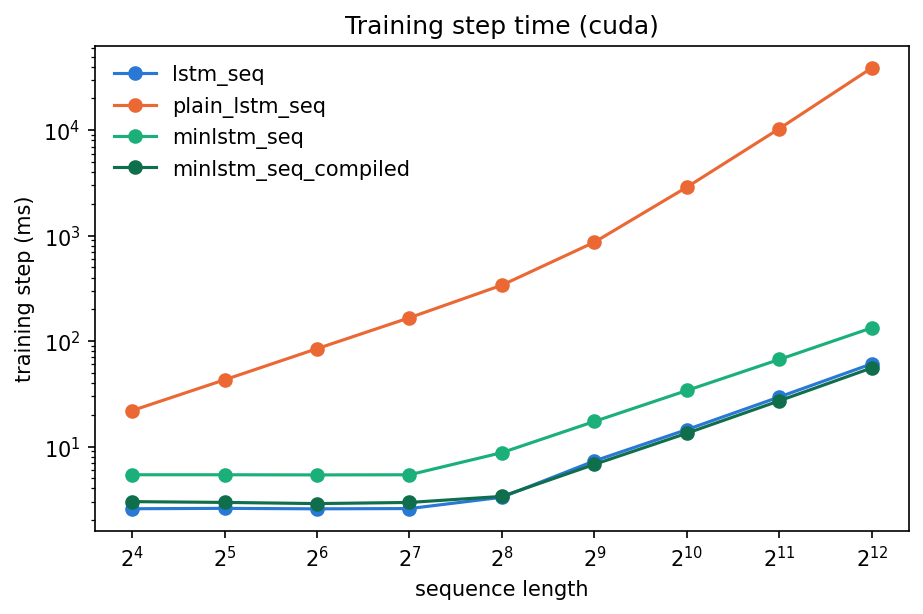
\includegraphics[width=\columnwidth]{../results/streaming_train_step.png}
  \caption{Training-step time versus sequence length.}
  \label{fig:train-step}
\end{figure}
Fig.~\ref{fig:train-step} shows training-step time for sequences of 16 to
4096 slots. Up to 256 slots, both cuDNN LSTM and compiled minLSTM take about
3\,ms per step, a cost set by fixed per-step overhead rather than by sequence
length. Beyond that, time grows linearly for every model, but at different
rates. The plain LSTM, which steps through time one slot at a time, takes
39\,s per step at 4096 slots. Compiled minLSTM takes 56\,ms, about
700$\times$ less. From 512 slots on, compiled minLSTM needs 7--9\% less time
than cuDNN LSTM (55.7 vs.\ 60.9\,ms at 4096), without a hand-written fused
kernel. In eager mode the scan is about 2.2$\times$ slower than cuDNN, so the
compiler is needed for this result. Compiled minLSTM also needs half the peak
memory of cuDNN LSTM (1.1 vs.\ 2.3\,GB at 4096 slots).

Table~\ref{tab:compute} gives per-slot inference cost. Streaming is what
matters most here. On the CPU, re-reading a 40-slot window costs
2.2--27$\times$ more than one streaming step, depending on the model. One minLSTM step takes 222\,$\mu$s
on the CPU, against 409\,$\mu$s for the library LSTM. A hand-written LSTM cell
is faster still (189\,$\mu$s), so at this size the CPU advantage reflects the
implementation as much as the architecture. On the GPU at batch 1, per-step
time is set by kernel-launch overhead rather than arithmetic, and minLSTM
(594\,$\mu$s), which launches more small kernels, is slower than cuDNN LSTM
(246\,$\mu$s). Every per-slot cost is below 0.6\,ms, far within the 100\,ms
slot. The clearest architectural advantage is arithmetic: a minLSTM layer
needs $3\,d_{\mathrm{in}} H$ multiply-accumulates per step against
$4(d_{\mathrm{in}}+H)H$ for LSTM, 12{,}800 vs.\ 49{,}792 here
(3.9$\times$ fewer). This matters on low-power accelerators where arithmetic,
not launch overhead, sets the cost.

\subsection{Beam misalignment versus array size}
\IfFileExists{tables/beam.tex}{\begin{table}[t]
\centering
\caption{Mean beam misalignment (half-power beamwidths) vs.\ array size.}\label{tab:beam}
\begin{tabular}{lrrrrr}
\toprule
Method & $N_t{=}8$ & $N_t{=}16$ & $N_t{=}32$ & $N_t{=}64$ & $N_t{=}128$ \\
\midrule
Reactive (hold) & 0.03 & 0.06 & 0.13 & 0.26 & 0.51 \\
Constant velocity & 0.05 & 0.10 & 0.21 & 0.42 & 0.83 \\
LS line fit & 0.01 & 0.03 & 0.05 & 0.10 & 0.20 \\
Kalman (CV) & 0.01 & 0.02 & 0.05 & 0.10 & 0.20 \\
IMM (CV+CT) & 0.01 & 0.02 & 0.04 & 0.08 & 0.17 \\
LSTM & 0.01 & 0.02 & 0.04 & 0.08 & 0.16 \\
minLSTM & 0.01 & 0.03 & 0.05 & 0.10 & 0.20 \\
minLSTM-res & 0.01 & 0.03 & 0.05 & 0.10 & 0.20 \\
IMM + LSTM & 0.01 & 0.02 & 0.04 & 0.08 & 0.16 \\
IMM + minLSTM & 0.01 & 0.02 & 0.04 & 0.08 & 0.17 \\
IMM + minLSTM-res & 0.01 & 0.02 & 0.04 & 0.08 & 0.17 \\
\bottomrule
\end{tabular}
\end{table}
}{\todo{run beam\_eval.py}}
Table~\ref{tab:beam} reports the mean misalignment in beamwidths. Because the
beamwidth shrinks as $1/N_t$, misalignment measured in beamwidths roughly
doubles each time the array doubles. Whether to predict matters far more than
which predictor to use. With 128 elements, holding the last observation leaves
a mean misalignment of 0.51 beamwidths, already past the half-beamwidth outage
threshold, and two-point extrapolation leaves 0.83. Every tracker stays below
0.21. Among trackers the spread is small: 0.167 beamwidths for the IMM, 0.156
for the LSTM correction and 0.167 for the minLSTM correction. Up to 64
elements, the IMM and every learned model are within 0.02 beamwidths of each
other, so their accuracy differences matter for beam alignment only with
very large arrays. Outage, the fraction of slots misaligned by more than half
a beamwidth, shows the same pattern. With 64 elements it is 13.6\% for the
reactive beam, 1.1\% for the IMM and 0.6\% for the LSTM correction. With 128
elements it is 28.2\%, 6.3\% and 5.8\%, while the minLSTM correction matches
the IMM at 6.3\%.

\section{Limitations and Future Work}
The trajectories are synthetic, and learned models may partly fit the
generator. The generator is also the coordinated-turn model with Markov-like
turn-rate switches, which is the model class the IMM assumes. The IMM is
therefore a strong reference here, and a learned correction has little room to
improve on it. Mobility the IMM does not model (stop-and-go, lane changes,
map-constrained turns) should leave more room. In the held-out-regime experiment the classical trackers are
re-tuned without the held-out regime. The networks, however, reuse
hyperparameters selected on a validation set that contains it, so their
held-out rows are mildly optimistic. Validation on DeepSense~6G~\cite{alkhateeb2023deepsense} real
position and beam measurements is the next step. Multi-step prediction (lead
time for beam training) and uncertainty-aware beam widening~\cite{beamguard2026}
are natural extensions. The carrier is 60\,GHz; extending to sub-THz requires
a corresponding ray-traced scenario.

\section{Conclusion}
We recast predictive beam tracking as a streaming problem and compared minLSTM
and LSTM with tuned classical trackers under splits that hold out whole
trajectories and whole mobility regimes. On coordinated-turn mobility, a tuned
IMM is hard to beat. Networks that predict position directly do not beat it
and can fail badly on unseen speeds. Networks that correct the IMM do better.
An LSTM correction lowers error by 4.6\% on seen regimes but loses up to 8\%
on an unseen one. A minLSTM correction matches the IMM and stays within 2.2\%
of it everywhere. minLSTM also trains 7--9\% faster than cuDNN LSTM on long
sequences once compiled, and runs one constant-cost update per slot at
inference. For deployment, this argues for learned corrections anchored on a
classical filter rather than end-to-end predictors. Validation on real
measurements is the next step. In beam terms, any predictive tracker keeps a
128-element beam within 0.21 beamwidths on average, against 0.51 for a
reactive beam. The IMM and its learned corrections differ by about 0.01
beamwidths.

\bibliographystyle{IEEEtran}
\bibliography{refs}

\end{document}
